\chapter{Fonctionnement et tests}

Dans cette partie nous chercherons à décrire dans un premier temps les fonctionnements ou, le cas échéant, les non fonctionnements de notre application. Nous aborderons ensuite la politique de test menée pour vérifier notre code. 

\section{Fonctionnement}

Afin d'introduire le fonctionnement des deux modules de l'application, nous avons réalisé deux diagrammes de séquences décrivant le fonctionnement global du programme :

\begin{figure}[!ht]
\begin{center}
  \fbox{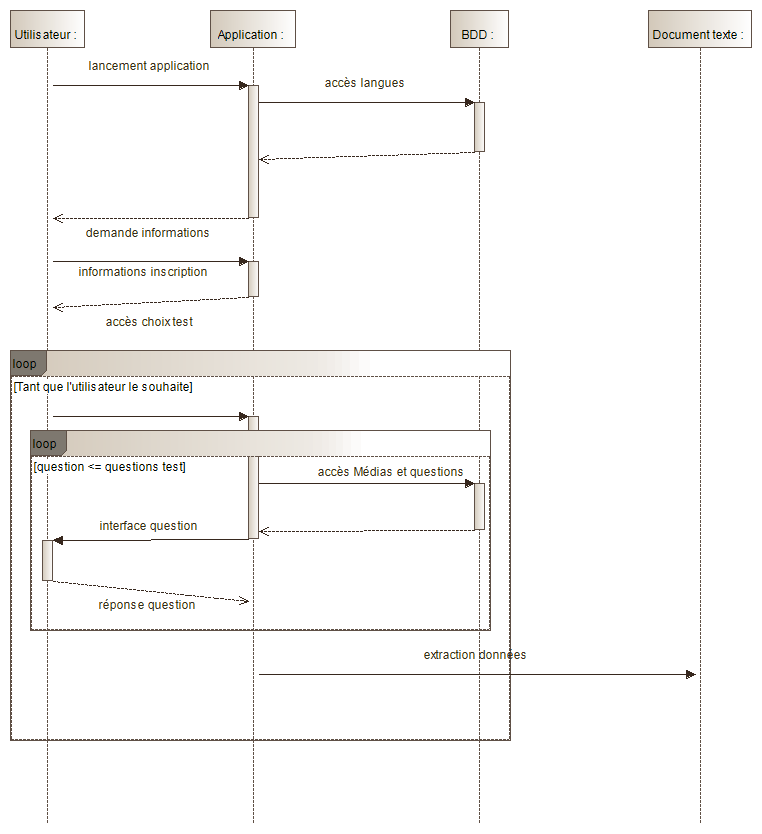
\includegraphics[width=10cm]{./fonctionnement_tests/sequence.png}}
  \caption{Fonctionnement - Fonctionnement interface graphique}
  \label{sequence} 
\end{center}
\end{figure}

\begin{figure}[!ht]
\begin{center}
  \fbox{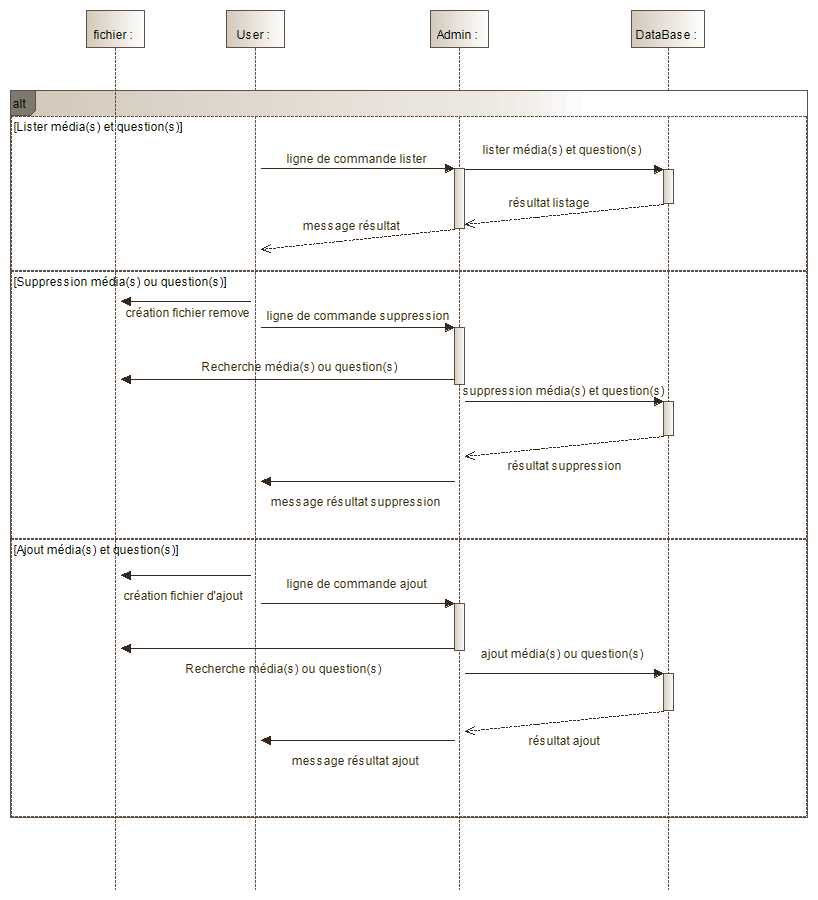
\includegraphics[width=10cm]{./fonctionnement_tests/sequenceAdmin.png}}
  \caption{Fonctionnement - Fonctionnement administration}
  \label{seqenceAdmin} 
\end{center}
\end{figure}

\newpage
L'application est séparée en deux modules, qui sont le module de test prosodique contenant l'interface graphique, et un module d'administration utilisable en ligne de commande. Ces deux modules partagent la même BDD. Ils sont donc, une fois compilés et compressés dans des \textit{jar}, situés dans le même répertoire, pour accéder à une BDD commune. Afin de garder une organisation des fichiers qui seront créés ou importés, nous avons codé un script organisant des fichiers de l'application lors de sa première utilisation. Ce script crée les répertoires avec l'arborescence suivante :

\begin{figure}[!ht]
\begin{center}
  \fbox{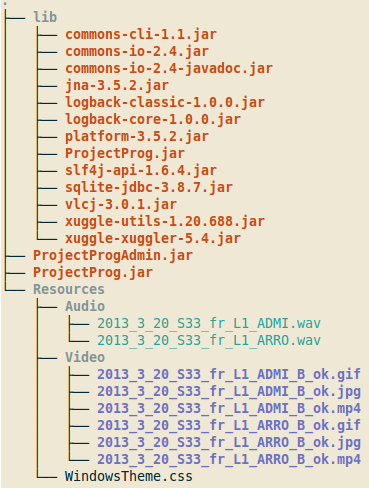
\includegraphics[width=5cm]{./fonctionnement_tests/tree.png}}
  \caption{Fonctionnement - Organisation répertoires}
  \label{tree} 
\end{center}
\end{figure}

Il est bien évident qu'avant toute utilisation du test prosodique, l'administrateur doit remplir la BDD avec des vidéos, des audios et des questions, sans quoi la BDD sera vide, et le test prosodique impossible.

Lorsque l'on lance l'application de test prosodique, on exécute l'interface graphique (dans le package \textit{GUI}). Cette interface fait appel aux autres parties de l'architecture pour afficher et organiser ses composants.

\subsection{Interface Graphique (GUI)}\label{GUI}

Tout d'abord, nous allons expliquer notre choix de technologie, qui s'est orienté vers le \textit{JavaFX}.
Nous pensions dans un premier temps développer l'application en deux étapes séparées : une première partie en \textit{Java} pour le côté traitement, puis une partie en \textit{Java EE} afin de pouvoir générer des pages \textit{HTML} pour l'interface graphique, et ainsi pouvoir complètement gérer l'apparence de notre application. 

Ensuite, après quelques recherches sur internet, nous avons découvert l'existance du \textit{JavaFX}.
Cette librairie de \textit{Java} est vue par ses créateurs comme l'évolution de \textit{Swing}.
Elle en est une évolution du fait du total contrôle que l'on a sur l'apparence de l'interface créée : contrairement à \textit{Swing}, où l'on utilise des composants inaltérables, tous les éléments sont personnalisables (boutons, arrière plan, police, organisation et taille des éléments).
Cette librairie était donc adaptée, car nous avions comme contrainte de développer une application ergonomique, ce qui n'est pas le cas d'une application développée avec \textit{Swing}, très limitée graphiquement.\\
\\


La méthode \textit{main} de Start.java est appelée lors du démarrage de l'application. Cette méthode fait créer une instance de UserGUI, la première page de l'application qui s'affiche.

\begin{figure}[!ht]
\begin{center}
  \fbox{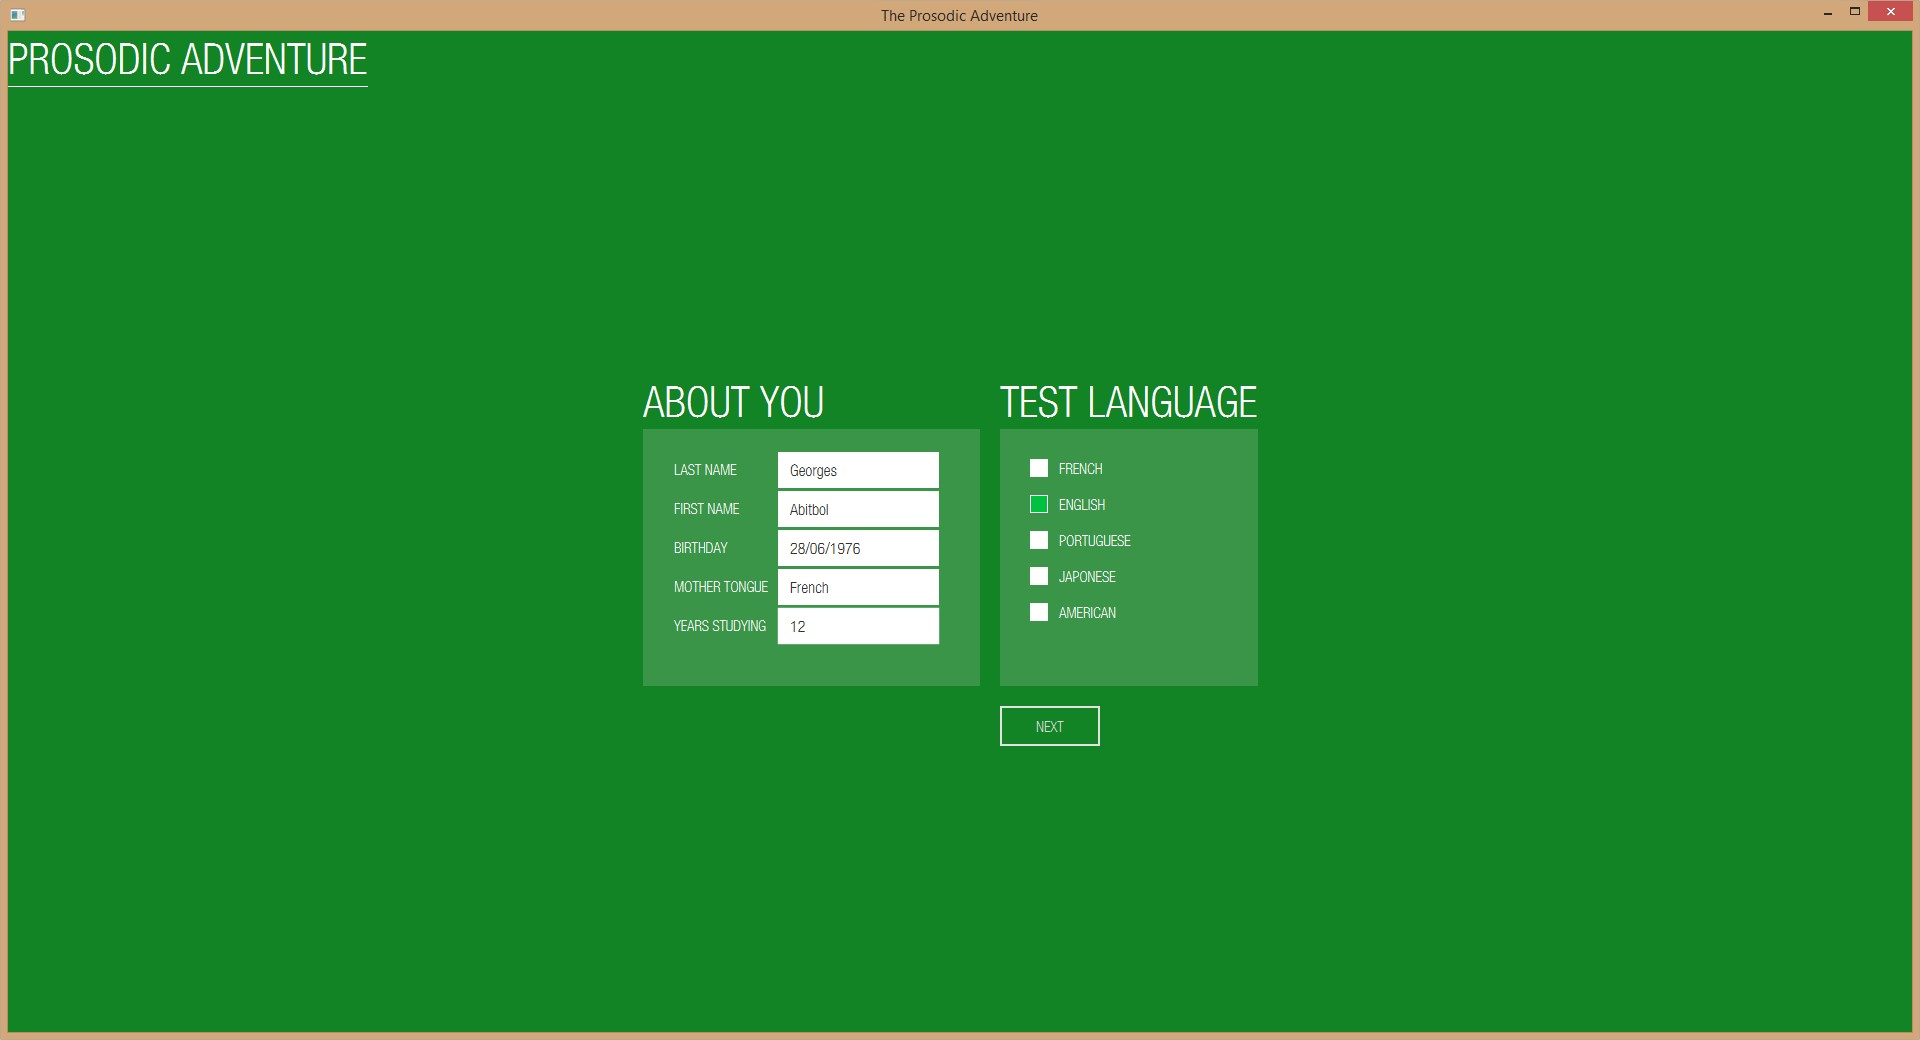
\includegraphics[width=8cm]{./fonctionnement_tests/UserGUI.jpg}}
  \caption{Fonctionnement - UserGUI}
  \label{UserGUI} 
\end{center}
\end{figure}

Pour récupérer les langues disponibles, UserGUI fait appel au contrôleur, dont nous décrirons le fonctionnement par la suite.
Les informations entrées par l'utilisateur dans les champs de ``\textsc{about you}'' (voir \textsc{Figure} \ref{UserGUI}) sont récupérées lors du clic sur le bouton ``\textsc{next}''. Ces données sont récupérées dans un fichier \textit{txt} par le biais du package \textit{Extract} que nous allons voir plus tard.

Après l'exportation des données sur l'utilisateur, un lien est fait vers la seconde page de l'interface : ChooseGUI (voir \textsc{Figure} \ref{ChooseGUI}). Cette page est une simple page avec deux boutons pour savoir dans quel mode veut aller l'utilisateur (apprentissage de l'application ou test concret).


\begin{figure}[!ht]
\begin{center}
  \fbox{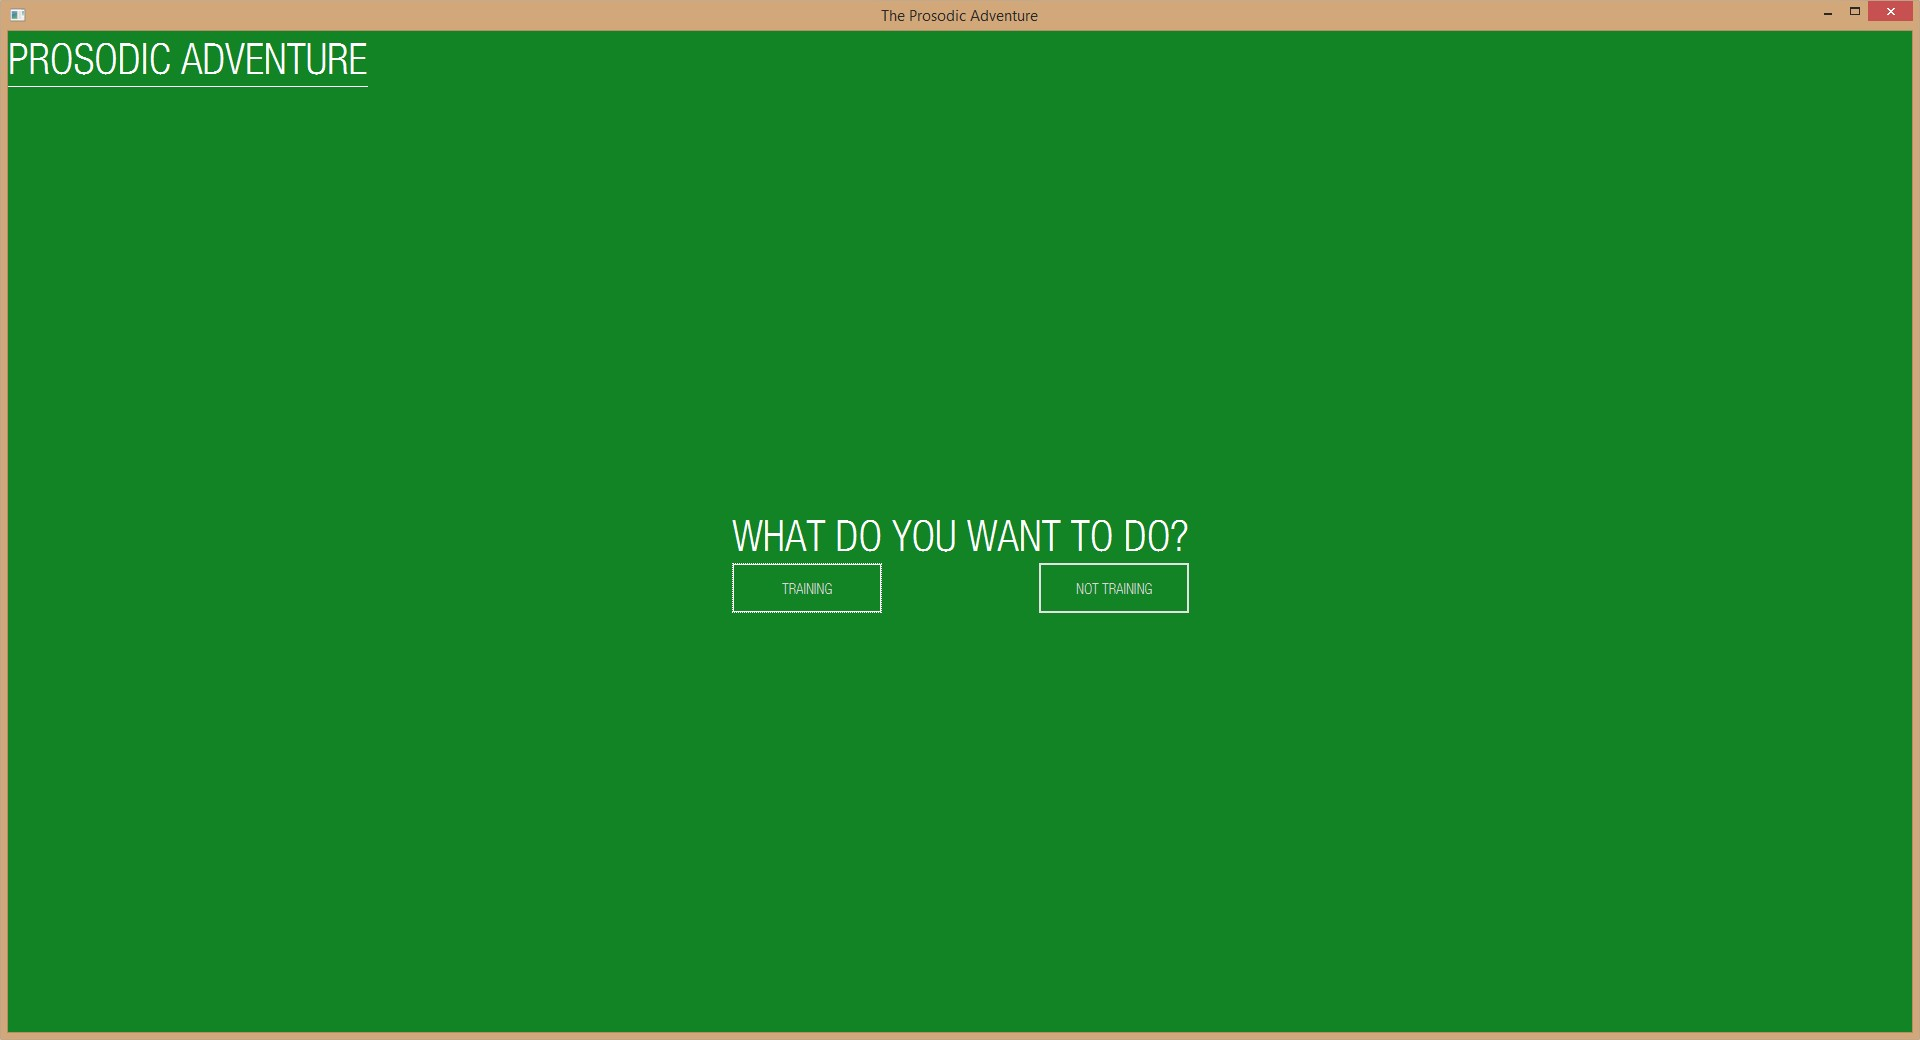
\includegraphics[width=8cm]{./fonctionnement_tests/ChooseGUI.jpg}}
  \caption{Fonctionnement - ChooseGUI}
  \label{ChooseGUI} 
\end{center}
\end{figure}

On est ensuite dirigé vers la page de test (identique dans le mode ``\textsc{training}'' et ``\textsc{not training}''). La seule différence entre les deux modes est l'exportation de données : dans le test réel, les données sont exportées tandis que dans le mode de découverte, rien n'est exporté.
Les données exportées sont :
\begin{itemize}
 \item Les questions posées
 \item La vidéo réponse
 \item L'audio réponse
\end{itemize}
Ces données sont exportées lors du passage à la question suivante.
Ces précédentes données sont un choix parmis plusieurs. Ces listes de choix sont sélectionnées par les sous-classes \textit{SonGUI}, \textit{VideoGUI} et \textit{QuestionGUI} qui font le lien vers le contrôleur (voir \ref{controller}) afin de récupérer les médias dans la base de données.

\begin{figure}[!ht]
\begin{center}
  \fbox{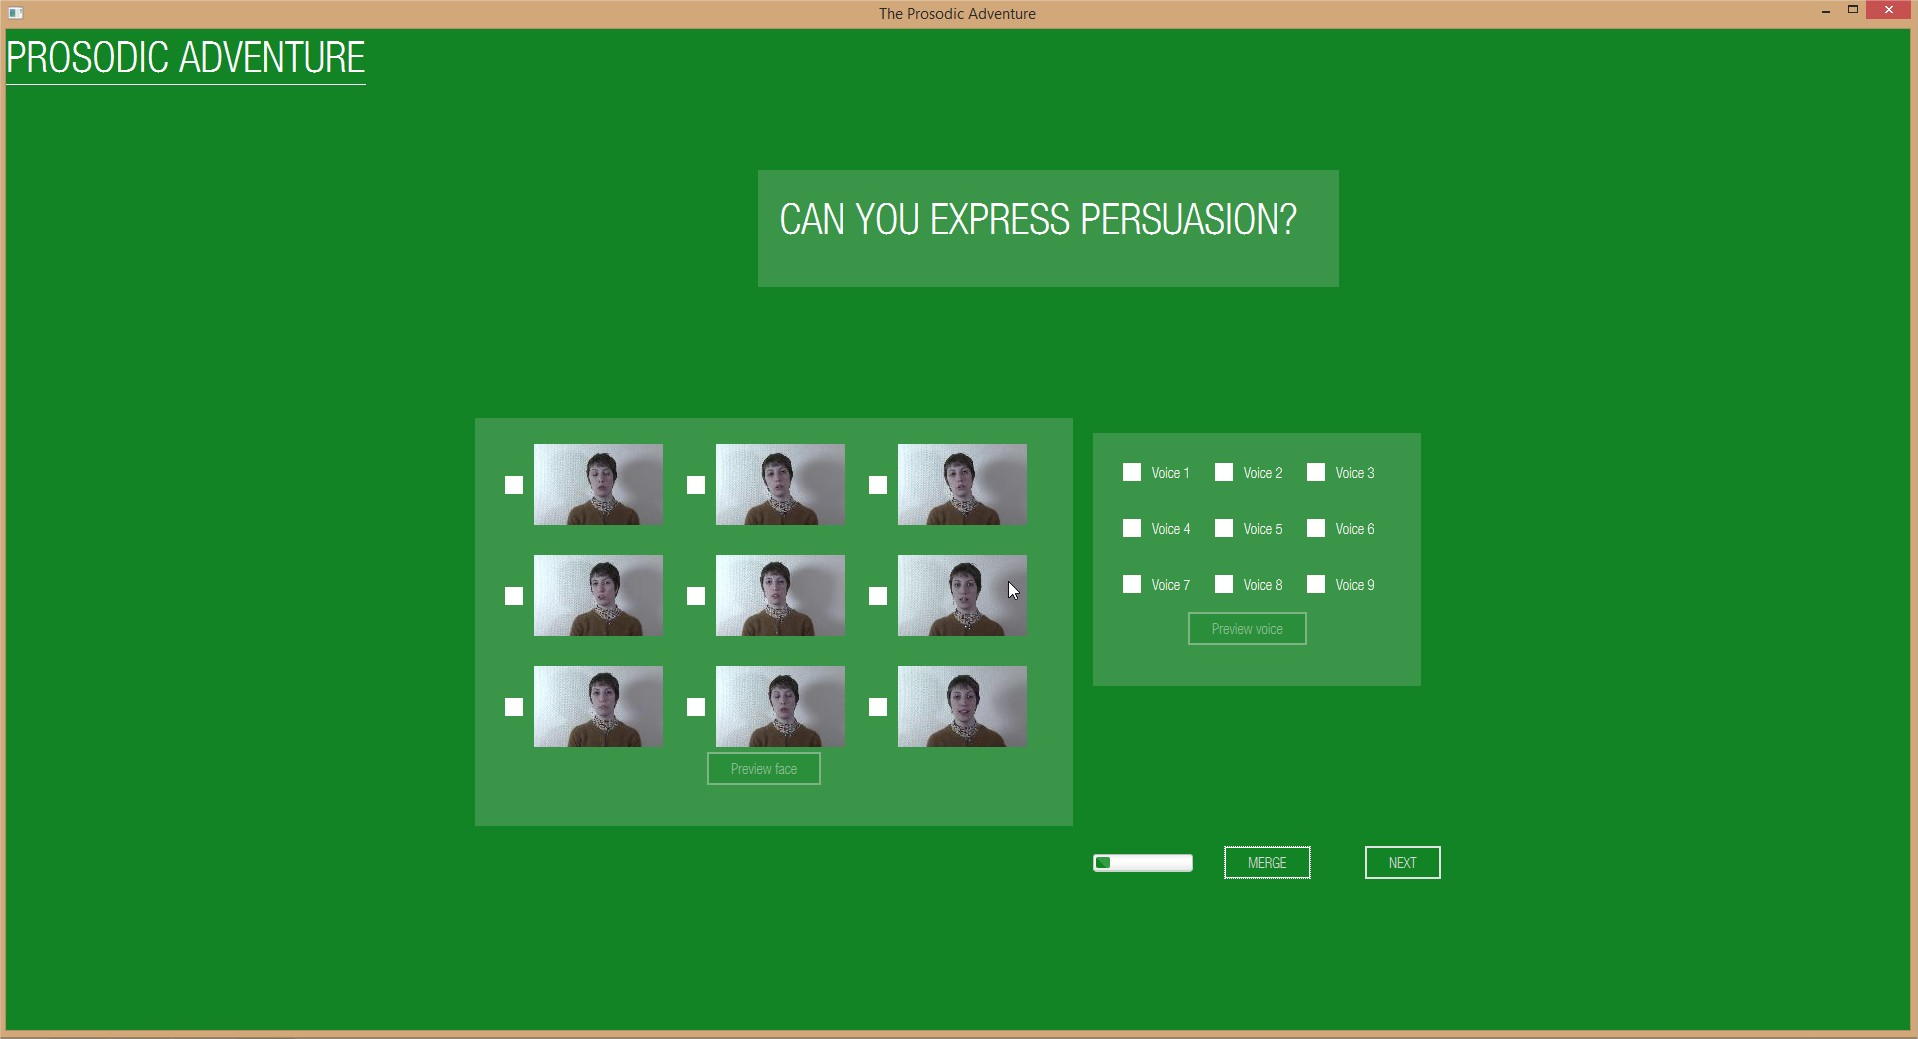
\includegraphics[width=8cm]{./fonctionnement_tests/TestGUI.jpg}}
  \caption{Fonctionnement - TestGUI}
  \label{TestGUI}
\end{center}
\end{figure}

Les boutons ``\textsc{preview}'' permettent de voir le contenu des vidéos et d'écouter les sons disponibles dans les différentes listes. Afin d'être joués, les médias sont ouverts (voir \textsc{Figure} \ref{VLC} avec VLC (en \textit{standalone}) en faisant appel à la librairie VLC inclue dans le projet (librairie implémentée dans la classe \textit{MediaPlayer}). Nous avons choisi d'utiliser ce lecteur de médias car le lecteur par défaut de \textit{JavaFX} est trop strict au niveau des codecs vidéos et audios qu'il accepte. VLC, quant à lui, nous offre la possibilité de lire la totalité des médias que l'on doit traiter. Ensuite, la stratégie du \textit{standalone} a été utilisée, car une intégration d'un lecteur non natif \textit{JavaFX} nécessite l'utilisation de la librairie \textit{Swing}, qui connait énormément de problèmes d'intégration à l'interface \textit{JavaFX}.

Ceci reste tout de même une voie intéressante d'amélioration. Nous avons nous même tenté de palier ce problème en convertissant les médias à la volée, en utilisant l'extension \textit{Xuggler}. Cependant, ceci demandait beaucoup de temps, et la duplication de tous les médias (ce qui n'est pas négligeable compte tenu de notre besoin d'avoir une application nomade, donc légère).

\begin{figure}[!ht]
\begin{center}
  \fbox{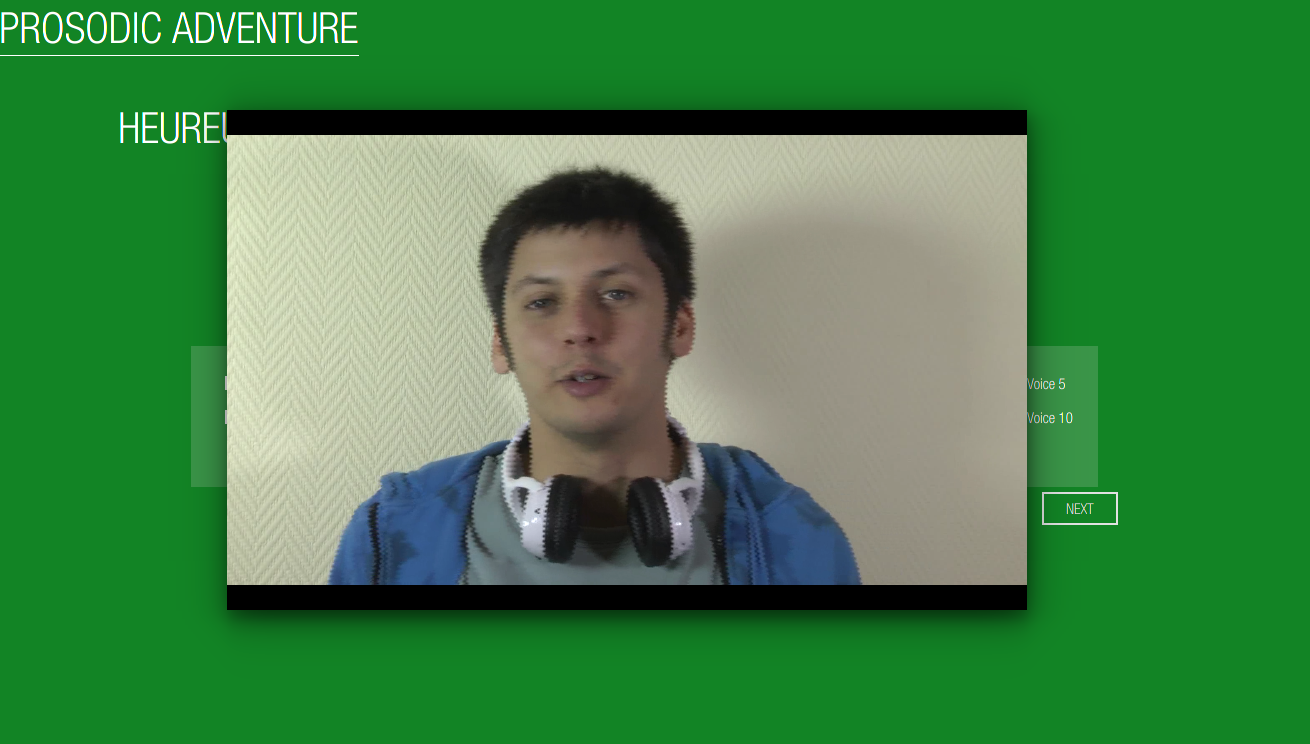
\includegraphics[width=8cm]{./fonctionnement_tests/VLC.png}}
  \caption{Fonctionnement - TestGUI}
  \label{VLC} 
\end{center}
\end{figure}

Finalement, une fois le test terminé, l'utilisateur est redirigé vers une page terminale contenant juste un message de remerciement, ainsi qu'un bouton ramenant vers la première page (\textit{UserGUI}).

\begin{figure}[!ht]
\begin{center}
  \fbox{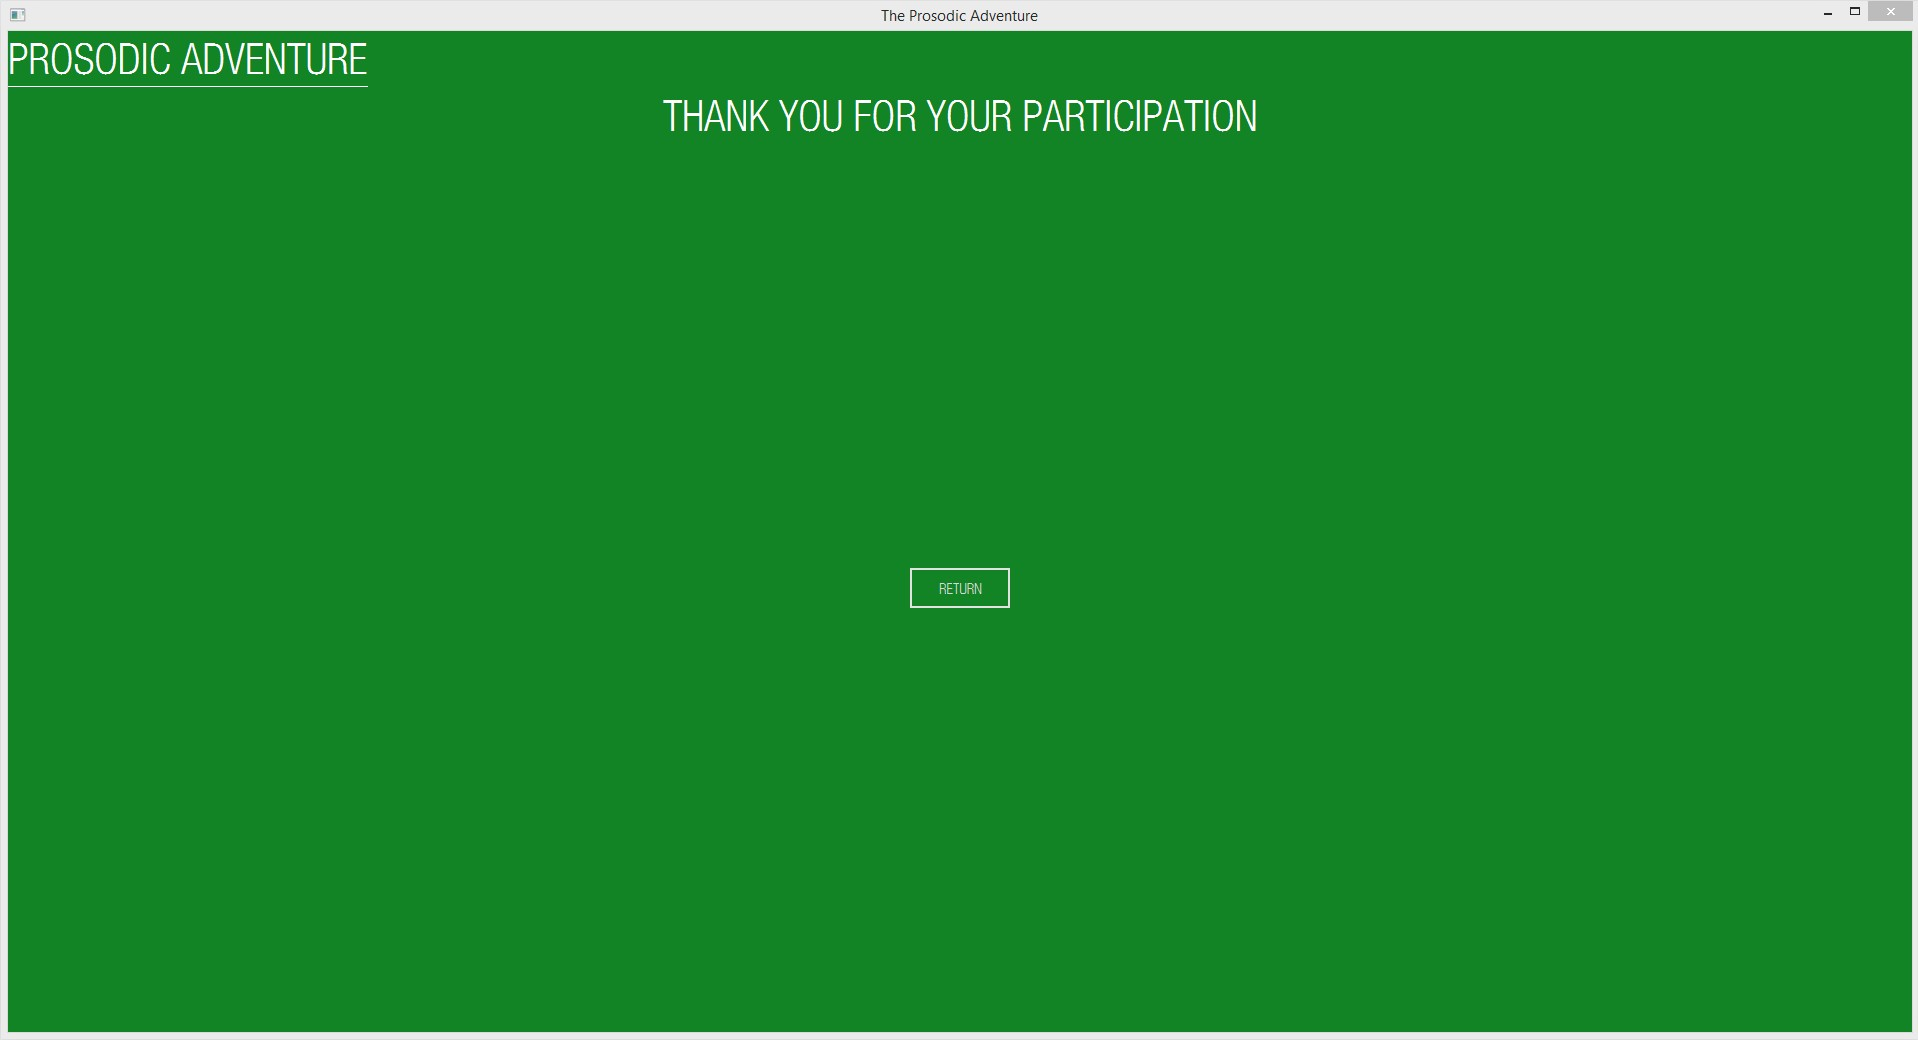
\includegraphics[width=8cm]{./fonctionnement_tests/EndGUI.jpg}}
  \caption{Fonctionnement - EndGUI}
  \label{endGUI} 
\end{center}
\end{figure}

\subsection{Base de données}\label{BDD}

Le système de gestion de base de données relationnelles (SGBDR) choisi a été \textit{SQLite}. Ce SGBDR est utilisable sur n'importe quelle plateforme, sans nécessiter l'installation et la mise en place d'un serveur. Il se résume à un fichier \textit{.db} qui contient toute la base de données.
Pour le fontionnement de l'application, l'implémentation de méthodes d'accès à la base de données a été necessaire :


\begin{itemize}
 \item Création de la base de données et de ses dépendances (si elle n'existe pas)
 \item Remplissage de la base de données
 \item Consultation du contenu de la base de données
 \item Recherche dans la base de données selon plusieurs critères
 \item Tirage au hasard d'un media de la base de données
 \item Suppression d'un media de la base de données, tout en vérifiant l'intégrité des relations (voir exemple plus en fin du paragraphe suivant)
\end{itemize}


Toutes ces implémentations sont fonctionnelles. Des tests ont été réalisés dessus (voir \ref{tests}).
Les accès à la base de données sont effectués par le driver\footnote{sqlite-jdbc-3.8.7} \textit{Java} de \textit{SQLite}.

Pour éviter tout conflit lors de l'accès à la base de données, des transactions manuelles ont été mises en place : un verrou est créé à chaque accès. Ainsi, un double accès ne peut pas être effectué.
Etant donné que \textit{SQLite} ne gère pas les contraintes de clé étrangère, nous avons établi un système de vérification en \textit{Java}. Elle inspecte chaque modification sensible (suppression d'une vidéo qui pourrait être liée à une question par exemple), qu'aucune dépendance ne sera brisée.


\subsection{Contrôleur}\label{controller}


Le contrôleur étant le lien entre la base de données (modèle) et l'interface graphique (vue), il est appelé à être utilisé à chaque échange entre la vue et le modèle.
Considérant la partie \ref{GUI}, on peut comptabiliser 3 appels :

\begin{itemize}
 \item Lors de l'affichage de UserGUI (\textsc{Figure} \ref{UserGUI}), pour retrouver les languages de test disponibles. L'appel est fait vers une méthode de la classe \textit{ControllerDatabse}, elle-même faisant le lien vers la bonne méthode du package \textit{BDD.DataBase}.
 \item Lors du chargement de la question dans \textit{TestGUI} (\textsc{Figure} \ref{TestGUI}), pour récupérer une question de la base de données, à partir des sous-classes de l'interface graphique citées dans \ref{GUI}. Cette récupération fait appel à la classe \textit{SelectMedia}, elle-même créant une liste de médias retournée par le package \textit{BDD}.
 \item Lors du passage à une question suivante dans l'interface graphique \textit{TestGUI}, car les réponses choisies par l'utilisateur sont récupérées, afin de générer une trace de son test. Ces réponses sont donc récupérées par la classe \textit{MediaSelected}, qui fait cette fois un lien vers le package \textit{Result}, que nous décrirons en \ref{export}.
\end{itemize}


\subsection{Exportation des données}\label{export}

Tout ce qui concerne l'exportation des données se situe dans le package \textit{Result}. Ce package est séparé en 
 éléments :
 
 \begin{itemize}
  \item \textit{Answer.java} qui permet de créer un objet \textit{Answer} afin de centraliser les données à extraire.
  \item \textit{User.java} qui a la même fonction que la classe précédente, mais qui contient les informations sur l'utilisateur (informations récupérées dans l'interface \textit{UserGUI}, voir \ref{GUI}).
  \item \textit{Extract} extrait les données contenues dans les deux précédents types d'objet, et les écrit dans un fichier texte, comme dans l'exemple suivant :
 \end{itemize}
 
 \begin{verbnobox}[\small]
  Langage:   French
  User:
      First Name:   Georges
      Last Name:   Abitbol
      Birthday   09/08/1979
      Mother Tongue   French
      Years learning tongue selected   1
  List of answers
      Answer 1:
	    Question:   Pouvez-vous exprimer la douleur avec ces audios et vidéos ?
	    Video   ADMI_B_ok
	    Audio   ADMI

 \end{verbnobox}
 
 
\subsection{Administration}\label{fonction_admi}

L'administration est une application qui fonctionne indépendamment de l'application graphique.
Elle est lancée en ligne de commande (\textit{java -jar <fichier.jar> <paramètre 0> <paramètre 1> <paramètre 2>}), les paramètres correspondants aux différentes fonctionnalités.
Nous avons décidé de créer nos propres arguments au lieu de laisser la possibilité à l'administrateur de lancer directement des requêtes \textit{SQL}. Ce choix a été fait afin d'éviter toute corruption involontaire de la BDD. Dans notre application, seuls les fichiers adaptés, avec les noms adaptés peuvent être ajoutés.
Ce besoin de contrôle de la nomenclature est nécessaire car nous extrayons l'ensemble des informations sur les médias (langue, format, titre du média) depuis leur nom.

Nous allons décrire le fonctionnement de cette application en partant des choix de paramètres possibles, récapitulés ci-dessous :

\begin{figure}[!ht]
\begin{center}
\begin{tabularx}{7cm}{|c|c|X|}
 \hline
 Paramètre 0 & Paramètre 1 & Paramètre 2\\
 \hline
	& video		& \tabularnewline
 add	& audio		& <fichier>\tabularnewline
	& question	& \tabularnewline
\hline
	& video		& \tabularnewline
 rm	& audio		& <fichier>\tabularnewline
	& question	& \tabularnewline
\hline
	& video		& \tabularnewline
 ls	& audio		& \tabularnewline
	& question	& \tabularnewline
 \hline
\end{tabularx}
\end{center}
\caption{Fonctionnement - Utilisation de l'application d'administration}
\end{figure}


\subsubsection{Paramètre ``add''}

L'ajout de contenu se fait par le biais d'un fichier (sans extension) contenant du simple texte.
Ce texte doit être formaté selon les règles suivantes :
\begin{itemize}
 \item Ajout de vidéos : le nom d'une vidéo par ligne, selon la syntaxe :
  \begin{verbnobox}[\small][0-9]*_[0-9]*_[0-9]*_[a-zA-Z0-9]*_[a-z]{2}_[a-zA-Z0-9]*_[a-zA-Z0-9]*.[a-zA-Z0-9]*\end{verbnobox}
  Comme par exemple :
 \begin{verbnobox}[\small]
  2013_3_20_S33_fr_L1_OBVI_B_ok.mp4
  2013_3_20_S33_fr_L1_SEDU_B_ok.mp4
  2013_3_20_S33_fr_L1_SINC_B_ok.mp4
 \end{verbnobox}
 \item Ajout d'audios : le nom d'un audio par ligne, selon la syntaxe :
  \begin{verbnobox}[\small][0-9]*_[0-9]*_[0-9]*_[a-zA-Z0-9]*_[a-z]{2}_[a-zA-Z0-9]*_[a-zA-Z0-9]*.[a-zA-Z0-9]*\end{verbnobox}
  Comme par exemple :
 \begin{verbnobox}[\small]
  2013_3_20_S33_fr_L1_OBVI.wav
  2013_3_20_S33_fr_L1_SEDU.wav
  2013_3_20_S33_fr_L1_SINC.wav
 \end{verbnobox}
 \item Ajout de questions : par groupe de trois lignes avec :
  \subitem Première ligne  : contenu de la question
  \subitem Seconde ligne   : vidéo attendue en réponse (avec la même syntaxe que lors de l'ajout de vidéos)
  \subitem Troisième ligne : audio attendu en réponse (avec la même syntaxe que lors de l'ajout d'audios)
  \subitem Comme par exemple :
 \begin{verbnobox}[\small]
  Can you express empathy?
  2013_3_20_S33_fr_L1_SEDU_B_ok.mp4
  2013_3_20_S33_fr_L1_SINC.wav
  Can you express pleasure?
  2013_3_20_S33_fr_L1_SURP_B_ok.mp4
  2013_3_20_S33_fr_L1_SINC.wav
 \end{verbnobox}
\end{itemize}

Ces ajouts font appel à une méthode d'ajout de médias, sachant de quel type de média il s'agit. Cette méthode rempli la BDD après avoir appelé une méthode d'extraction des données du fichier passé en paramètre à l'aide de \textit{regex}.

\subsubsection{Paramètre ``rm''}

La suppression de contenu se fait d'une manière similaire à l'ajout : une méthode est chargée de la suppression en BDD des médias, faisant elle-même appel à la fonction d'extraction des données, pour identifier les tuples à supprimer. Ensuite, une fonction gestion de l'intégrité de la BDD vérifie que ces médias ne sont pas liés à une question encore existante.

Seule la suppression de question diffère de l'ajout : seul le nom des questions doit être entré dans le fichier passé en paramètre. Le fonctionnement reste ensuite identique à la suppression de vidéos ou d'audios.

\subsubsection{Paramètre ``ls''}

Comme dans un terminal \textit{Shell}, le paramètre \textbf{ls} permet de lister le contenu de la BDD. Pour afficher ce contenu, une méthode fait appel à la méthode de listage de toute une table de la BDD dans la classe \textit{DataBase}, du package \textit{BDD} de l'application graphique.

\section{Tests}\label{tests}

\subsection{Fonctionnels}

\subsubsection{Unitaires}

Pour réaliser les tests unitaires sur la base de données, nous avons utilisé le plugin \textit{JUnit}, disponible par défaut dans l'IDE \textit{Netbeans}.
Ce plugin permet de tester chaque méthode, afin de détecter d'éventuels problèmes d'implémentation.

Ces tests unitaires ont été effectués majoritairement dans le modèle (voir \ref{modele}), en particulier sur la classe \textit{Database}, cœur de la gestion des données. La seconde partie de ces tests a été faite dans le contrôleur (voir \ref{archi_controller}), sur les classes \textit{SelectMedia} et \textit{MediaSelected} lors des créations de listes de médias.

\paragraph{Boîte noire}

Les tests boites noires avec \textit{JUnit} correspondent aux tests d'entrée-sortie. On teste chaque méthode, on donne un objet en entrée et on vérifie que l'objet en sortie est bien le résultat attendu.

\paragraph{Boîte blanche}

Les tests boites blanches avec \textit{JUnit} permettent de vérifier les différents cas d'utilisation d'une fonction (par exemple, la méthode \textit{addVideo} ajoute une vidéo dans la BDD seulement si celle-ci n'existe pas encore).


Afin de contrôler l'efficacité de nos tests, nous avons utilisé un plugin disponible de \textit{Netbeans} (\textit{TikiOne JaCoCoverage Plugin}). Ce plugin surligne en vert (zones parcourues), jaune (zones parcourues, mais pas dans toutes les branches) ou rouge (zones non-parcourues, les erreurs en général), selon les zones de codes parcourues par les tests (voir \textsc{Figure} \ref{cocojava}).

\begin{figure}[!ht]
\begin{center}
  \fbox{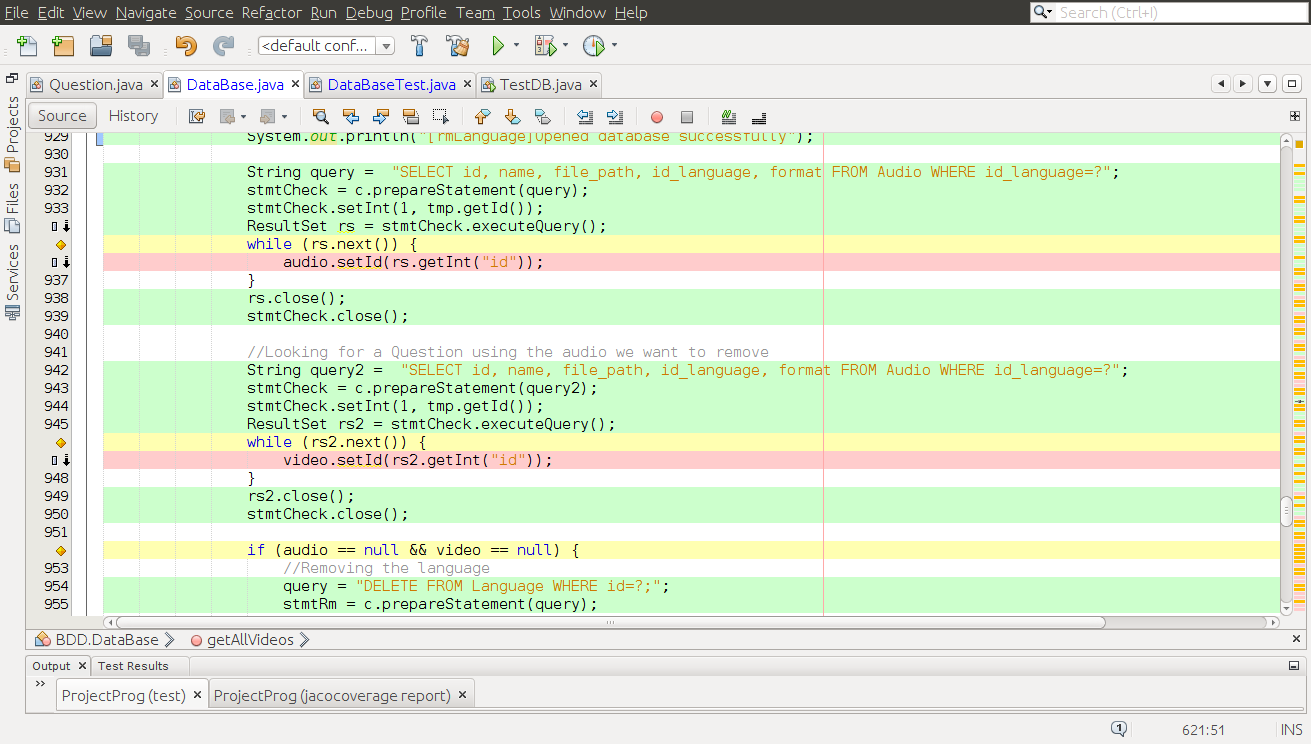
\includegraphics[width=12cm]{./fonctionnement_tests/CoCoJava.png}}
  \caption{Tests - Recouvrement des tests}
  \label{cocojava} 
\end{center}
\end{figure}


\subsection{Performances}

Afin de réaliser les tests de performance, nous avons simplement utilisé un plugin de \textit{Netbeans} (\textsc{Figure} \ref{perf}). Ce plugin permet de mesurer les performances en temps CPU.

Sachant déjà que nous avions un problème de performance pendant le chargement de la page \textit{TestGUI} (voir \ref{GUI}), ce test nous a permis d'identifier le code fautif.
Ainsi, l'accès à la base de données a été mis en cause. La méthode de connexion étant seulement gérée par le driver \textit{SQLite-jdbc}, nous pouvons donc en conclure que notre gestion des accès à la BDD n'est pas optimisée.
Une piste d'amélioration serait de modifier le moment d'accès à la base de données. Il serait facilement envisageable de cloner la totalité de la BDD au lancement de l'application avec le pattern \textit{DAO (Data Access Object)}. Ce pattern permet de créer une séparation entre la BDD et l'application. L'application n'accède pas directement à la base de données, mais à une réplique formée d'objets.
Ainsi, le chargement de toute la BDD étant fait au lancement de l'application, plus aucune latence ne se ferait ressentir, vu que les accès en BDD n'existeraient plus, pour laisser la place à l'accès à des objets beaucoup plus rapide.
De plus, notre architecture récupérant les informations de la BDD, en ayant une table correspondant à un type d'objet, facilite la transition vers un tel pattern.

\begin{figure}[!ht]
\begin{center}
  \fbox{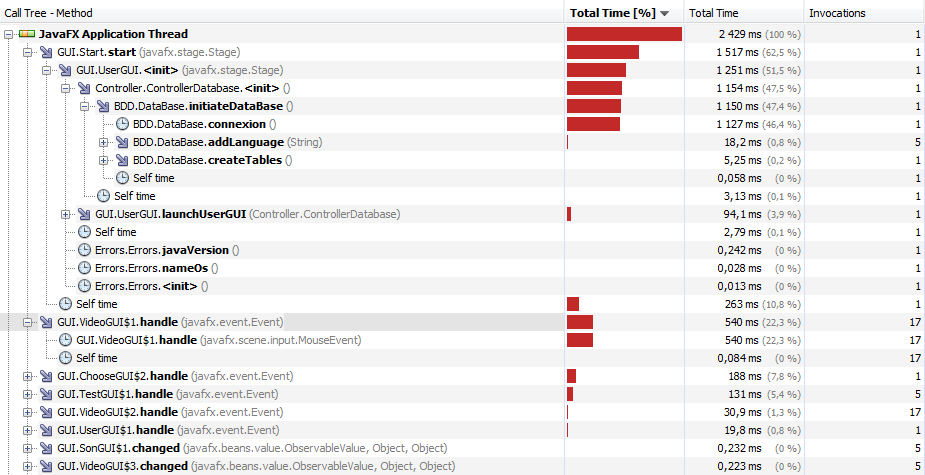
\includegraphics[width=12cm]{./fonctionnement_tests/performance.png}}
  \caption{Tests - Performances}
  \label{perf} 
\end{center}
\end{figure}






